\documentclass[a4paper,14pt,russian]{extreport}
\usepackage[russian]{babel}

\usepackage{../common/dsturep_ru} % оформление по ДСТУ 3008-95
\usepackage{import}
\usepackage{standalone}
\usepackage{comment}
\usepackage{bbm}

\usepackage{tikz}
\usepackage{tikz-3dplot}
\usetikzlibrary{calc}
\usetikzlibrary{plotmarks}
\usepackage{pgfplots}

%\usepackage{scrextend}
\usepackage{changepage}
\usepackage{caption}
\usepackage{listings}
%\usepackage[title,titletoc]{appendix}
%\usepackage{appendix}
\usepackage{longtable}
%\usepackage{slashbox}
\usepackage{diagbox}
\usepackage{lscape}
\usepackage{algorithmic}
\usepackage{algorithm}

\def\male{male}
\def\female{female}

\bibliographystyle{../common/utf8gost780u}

\usepackage[square,numbers,sort&compress]{natbib}
\renewcommand{\bibnumfmt}[1]{#1.\hfill} % нумерация источников в самом списке — через точку

\def\passYear{2017}
\def\faculty{физико-технический институт}
\def\department{Кафедра информационной безопасности}
\def\departmentHead{Н. В. Грайворонский}
\def\kind{Дипломна робота}
\def\level{магістр}
\def\specialityCode{8.04030101}
\def\specialityTitle{Прикладная математика}
\def\theme{Решение нелинейных уравнений}
\def\gender{female}
\def\mentorGender{male}
\def\course{3}
\def\group{ФИ-41}
\def\name{Лавягина Ольга Алексеевна}
\def\mentorRank{}
\def\mentorName{Стёпочкина Ирина Валерьевна}
\def\reviewerRank{Rank}
\def\reviewerName{Name}
\def\subject{Методы вычислений}



\begin{document}

\import{1_title/}{title.tex}

\clearpage

\pagenumbering{gobble}
%\import{3_abstract/}{main.tex}

\pagestyle{empty}
\thispagestyle{empty}
\tableofcontents

\clearpage
\pagenumbering{arabic}
\pagestyle{fancy}
\setcounter{page}{2}

\clearpage

\chapter{Задание}

Задана функция
$$ f \left( x \right) =
  \frac{1}{ \sin x}$$
на отрезке
$$ \left[ \frac{ \pi }{6}, \frac{ \pi }{2} \right].$$

Нужно построить таблицу значений функции в узлах на заданном отрезке.

По таблично заданной:
\begin{itemize}
  \item построить интерполяционный полином в форме Ньютона или Лагранжа;
  \item совершить интерполяцию спланами (второго или третьего порядка);
  \item построить график погрешности интерполяции
  $ \varepsilon = \left| P_n \left( x \right) - f \left( x \right) \right| $.
  Нужно вывести на график с шагом, меньше в 5-6 раз, чем шаг интерполяции,
  соответственные значения полинома, сплайн-функции и точной функции.
  Если погрешность очень мала, применить масштабирование.

  Сравнить полученный результат с теоретической оценкой погрешности.
\end{itemize}

\chapter{Интерполяционный полином с обозначением узлов интерполяции}

Пусть на
$$ \left[ \frac{ \pi }{6}, \frac{ \pi }{2} \right] $$
задана $n + 1$ точка ---
узлов интерполяции $x_0, x_1, \dotsc, x_n$ и значений функции в этих узлах
$f \left( x_0 \right), f \left( x_1 \right), \dotsc, f \left( x_n \right) $.

\lstset{inputencoding=utf8, extendedchars=\true}
\lstinputlisting[language=bash,
                 basicstyle=\ttfamily\scriptsize]{../code/table}

Нужно построить интеполяционный полином по этой таблице значений.

Необходимо, чтобы $L_n \left( x_i \right) = y_i$.
Отсюда
$$L_n \left( x \right) =
  \sum \limits_{i = 0}^n
    y_k \cdot
    \frac{ \left( x - x_0 \right) \dotsc \left( x - x_{k - 1} \right) \left( x - x_{k + 1} \right) \dotsc \left( x - x_n \right) }{ \left( x_k - x_0 \right) \dotsc \left( x_k - x_{k - 1} \right) \left( x_k - x_{k + 1} \right) \dotsc \left( x_k - x_n \right) }.$$

Для заданной таблицы
\lstset{inputencoding=utf8, extendedchars=\true}
\lstinputlisting[language=bash,
                 basicstyle=\ttfamily\scriptsize]{../code/lagrange}

Полученный полином изображён на рисунке \ref{fig:lagrange}.
Красным изображены узлы интерполяции.

\begin{figure}[h!]
  \centering
  \includegraphics[width=.4\textwidth]{../code/lagrange.png}
  \caption{Полином Лагранжа}
  \label{fig:lagrange}
\end{figure}

Для данных узлов получен интерполяционный полином Ньютона (рис. \ref{fig:newton}).

\begin{figure}[h!]
  \centering
  \includegraphics[width=.4\textwidth]{../code/newton.png}
  \caption{Полином Ньютона}
  \label{fig:newton}
\end{figure}

\chapter{Интерполирующая сплайн-функция}

Составлена ЛСУ для нахождения коэффициентов при сплайн-функции.
Использовано то, что все
$$h =
  \frac{ \pi }{30}.$$
Система имеет вид $Am = b$, где матрица $A$ имеет вид
$$A =
  \begin{bmatrix}
    \frac{ \pi }{45} & \frac{ \pi }{180} & 0 & 0 & 0 & 0 & 0 & 0 & 0 \\
    \frac{ \pi }{180} & \frac{ \pi }{45} & \frac{ \pi }{180} & 0 & 0 & 0 & 0 & 0 & 0 \\
    0 & \frac{ \pi }{180} & \frac{ \pi }{45} & \frac{ \pi }{180} & 0 & 0 & 0 & 0 & 0 \\
    0 & 0 & \frac{ \pi }{180} & \frac{ \pi }{45} & \frac{ \pi }{180} & 0 & 0 & 0 & 0 \\
    0 & 0 & 0 & \frac{ \pi }{180} & \frac{ \pi }{45} & \frac{ \pi }{180} & 0 & 0 & 0 \\
    0 & 0 & 0 & 0 & \frac{ \pi }{180} & \frac{ \pi }{45} & \frac{ \pi }{180} & 0 & 0 \\
    0 & 0 & 0 & 0 & 0 & \frac{ \pi }{180} & \frac{ \pi }{45} & \frac{ \pi }{180} & 0 \\
    0 & 0 & 0 & 0 & 0 & 0 & \frac{ \pi }{180} & \frac{ \pi }{45} & \frac{ \pi }{180} \\
    0 & 0 & 0 & 0 & 0 & 0 & 0 & \frac{ \pi }{180} & \frac{ \pi }{45} \\
    0 & 0 & 0 & 0 & 0 & 0 & 0 & 0 & \frac{ \pi }{180}
  \end{bmatrix},$$
вектор-столбец $b$ имеет вид
$$b =
  \begin{bmatrix}
    0.87732554713739574 \\
    0.55368012000205091 \\
    0.37508747138267329 \\
    0.26926450461833418 \\
    0.20343037684714838 \\
    0.16128958271650951 \\
    0.1341907730636353 \\
    0.11735430490342991 \\
    0.10813657580708488 \\
    0.10520039045588443
  \end{bmatrix}$$

Проведена интерполяция функции кубическим сплайном кубическим сплайном (рис. \ref{fig:spline}).

\begin{figure}[h!]
  \centering
  \includegraphics[width=.4\textwidth]{../code/spline.png}
  \caption{Кубический сплайн}
  \label{fig:spline}
\end{figure}

\chapter{Значение погрешности}

Погрешности были найдены в узлах, которые отстают друг от друга на
$$ \frac{ \pi }{150}$$
на отрезке
$$ \left[ \frac{ \pi }{6}, \frac{ \pi }{2} \right] $$
для всех использованных типов интерполяции.
Была использована формула
$$ \left| f \left( x \right) - polynom \left( x \right) \right|.$$
На рисунке \ref{fig:lerror} изображена погрешность для интеплоляции полиномом Лагранжа,
на рисунке \ref{fig:nerror} --- для полинома Ньютона, на риснке \ref{fig:serror} ---
для интерполяции кубическими сплайнами.

\begin{figure}[h!]
  \centering
  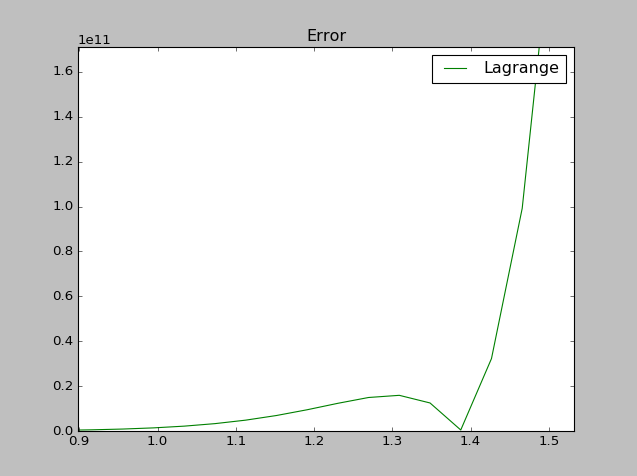
\includegraphics[width=.4\textwidth]{../code/lagrange_error.png}
  \caption{Погрешность для полинома Лагранжа}
  \label{fig:lerror}
\end{figure}

\begin{figure}[h!]
  \centering
  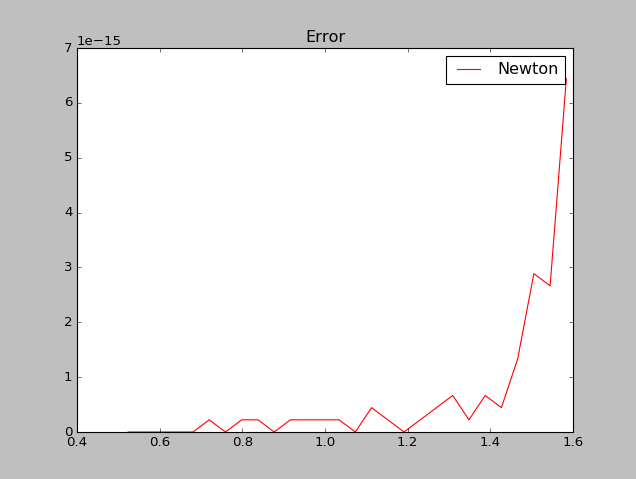
\includegraphics[width=.4\textwidth]{../code/newton_error.png}
  \caption{Погрешность для полинома Ньютона}
  \label{fig:nerror}
\end{figure}

\begin{figure}[h!]
  \centering
  \includegraphics[width=.4\textwidth]{../code/spline_error.png}
  \caption{Погрешность для сплайнов}
  \label{fig:serror}
\end{figure}

\chapter{Листинг программы}

Листинг файла \_\_main\_\_.py
\lstset{inputencoding=utf8, extendedchars=\true}
\lstinputlisting[language=python,
                 basicstyle=\ttfamily\scriptsize]{../code/__main__.py}

Листинг файла lagrange.py с вычислением интерполяционного полинома Лагранжа
\lstset{inputencoding=utf8, extendedchars=\true}
\lstinputlisting[language=python,
                 basicstyle=\ttfamily\scriptsize]{../code/lagrange.py}


Листинг файла newton.py с вычислением интерполяционного полинома Ньютона
\lstset{inputencoding=utf8, extendedchars=\true}
\lstinputlisting[language=python,
                 basicstyle=\ttfamily\scriptsize]{../code/newton.py}

Листинг файла spline.py с вычислением вектора-столбца $b$ для системы $Am = b$,
с помощью которой находятся коэффициенты $m$ сплайн-функции
\lstset{inputencoding=utf8, extendedchars=\true}
\lstinputlisting[language=python,
                 basicstyle=\ttfamily\scriptsize]{../code/spline.py}


\chapter*{Выводы}
\addcontentsline{toc}{chapter}{Выводы}

К функции была применена интерполяция методами Лагранжа, Ньютона, сплайнов.
Для этого были составлены узлы интерполяции на отрезке и найдены значения функции в этих узлах.

Построены графики погрешностей для данных методов, которые получились незначительными.
Интерполяция сплайнами дала наилучший результат.

\end{document}
